\section{Introduction}
As IO bandwidth continues to be significantly less than compute, in-situ frameworks have become essential in the modern HPC environment. Further, machine learning (ML) has become a signficant driving force within the HPC community, particularly to help analyze this ever increasing amounts of data. However, machine learning is predicated on the notion that programs or algorithms are constructed by combining data with output, which is the inverse of traditional programming: data and an algorithm generate output (Fig.~\ref{fig:ml-vs-trad}). Therefore, resources must be utilized to develop machine learning algorithms. 

To generate sophisticated machine learning algorithms often requires a significant amount of computation as well as copious amounts of output as input. The purpose of this project is then to offer a solution which provides the means necessary to design machine learning implementations at scale and in situ to aid or be the basis of scientific visualisation tasks. We accomplish this by providing read, write and in place data transfer functionality between learning models and visualisation task implementations. To our knowledge, this is the first scientific visualization-machine learning in-situ framework.

\begin{figure}
    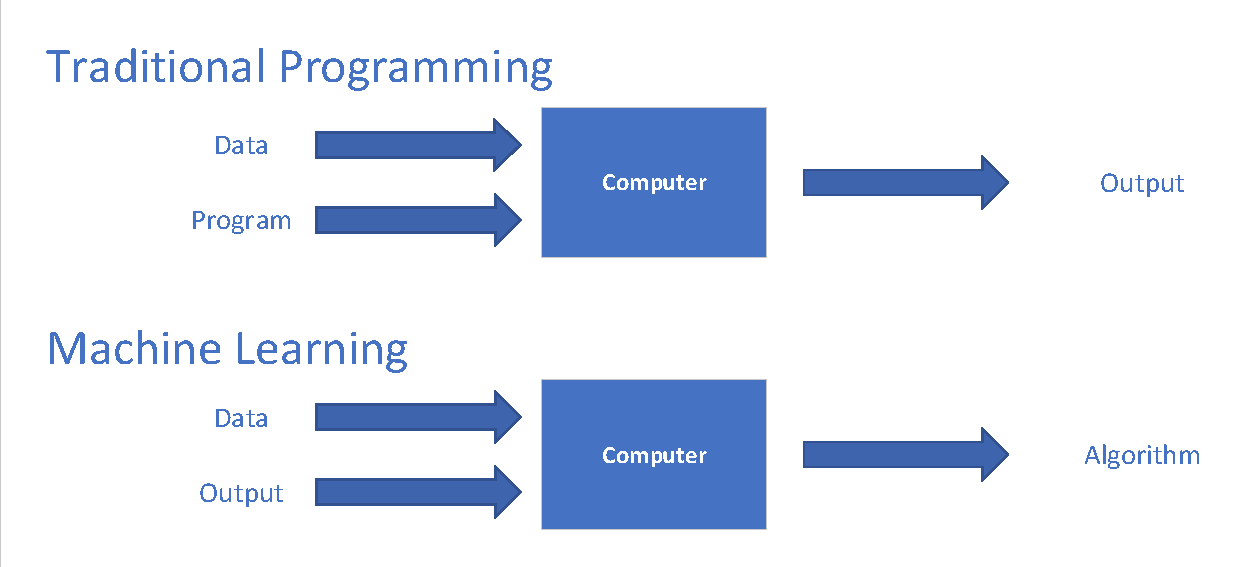
\includegraphics[width=\linewidth]{ML-data-output-program}
    \caption{Traditional programming vs machine learning.}
    \label{fig:ml-vs-trad}
  \end{figure}

In this work we present PAVE, an in-situ framework for coupling scientific visualization and machine learning along with a case study of coupling a path tracer, an accurate light transport simulation, with a neural network to build a filter for real time rendering and accurate light transport. The provided model is a coalescence of the Visualisation Toolkit fit for Massively threaded architectures (VTK-m) and Python, an increasingly popular language within the machine learning community due to robust libraries available for neural networks such as PyTorch. The resulting work accomplishes this combination by utilising VTK-m to construct a path trace rendering tool able to fluidly and efficiently communicate to a cGAN by means of PAVE during training.   The resulting generative model serves as a real-time filter for rendering globally illuminated images which accurately approximate diffuse indirect illumination and soft shadows with quality comparable to offline approaches. 

\begin{figure*}
    \includegraphics[width=\linewidth]{buffer_results_teaser}
    \caption{Rendered Conditional Geometry Buffers ({\bf left set}) and artificial rendering with conditional generative adversarial neural network ({\bf right couple}) comparing ground truth path traced rendering ({\bf left}) with image generated ({\bf right}).}
  \end{figure*}
